\section{Classificazione Binaria}
\textbf{Descrizione di cosa andremo a fare:} utilizziamo il dataset IMDb Dataset.
Questo dataset è un Database compilato dagli utenti del sito. Le caratteristiche, in particolare, sono:
\begin{itemize}
    \item 50.000 recensioni
    \item circa 50\% positive e 50\% negative
    \item \textit{25.000} sono usate per il \textbf{training} e \textit{25.000} sono usate per il \textbf{testing}. Anche queste sono il 50\% positive e 50\% negative.
\end{itemize}

La task che faremo su questo dataset prende il nome di \textbf{sentimental
    analysis}, ovvero analisi del sentimento.

\textbf{Assunzione:} Ciò che stiamo facendo ha senso solamente se assumiamo \textit{che nel futuro avremo punti con una distribuzione abbastanza simile a quelli utilizzati per il training}.

La partizione di \textbf{test} è una partizione che non viene utilizzata per la
fase di training, ma viene utilizzata successivamente per controllare se il
modello si sta comportando bene nella predizione dei valori. Ci sono delle
misure che hanno range $[0,1]$ che ci permettono di capire quanto il modello si
sta comportando bene.

\textbf{Nota:} il \textit{test set} non viene fornito quando si lavora nel deep learning, altrimenti verrebbe usato per ottimizzare direttamente il modello. \textbf{Non si conosce inizialmente.}

% BEGIN: xz8c6549bwf9
\begin{figure}[H]
    \centering
    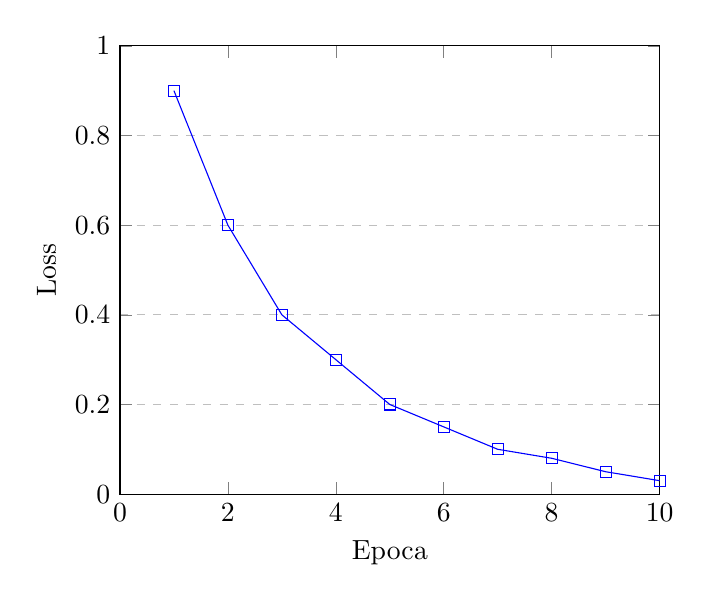
\begin{tikzpicture}
        \begin{axis}[
                xlabel={Epoca},
                ylabel={Loss},
                xmin=0, xmax=10,
                ymin=0, ymax=1,
                xtick={0,2,4,6,8,10},
                ytick={0,0.2,0.4,0.6,0.8,1},
                legend pos=north east,
                ymajorgrids=true,
                grid style=dashed,
            ]
            \addplot[
                color=blue,
                mark=square,
            ]
            coordinates {
                    (1,0.9)(2,0.6)(3,0.4)(4,0.3)(5,0.2)(6,0.15)(7,0.1)(8,0.08)(9,0.05)(10,0.03)
                };
        \end{axis}
    \end{tikzpicture}
    \caption{Grafico di una curva di loss che diminuisce all'aumentare delle epoche.}
    \label{fig:loss_curve}
\end{figure}
% END: xz8c6549bwf9

\subsection{Caricamento e gestione del Dataset}

\begin{lstlisting}[language=Python, caption=Caricamento del dataset IMDb Dataset.]
from keras.datasets import imdb
(train_data, train_labels), (test_data, test_labels) = imdb.load_data(num_words=10000)
\end{lstlisting}

\begin{itemize}
    \item training\_data: sono gli input del training
    \item training\_labels: sono gli output del training
    \item test\_data: sono gli input del test
    \item test\_labels: sono gli output del test
\end{itemize}

% BEGIN: 7z5t8f6d4xw3
\begin{figure}[H]
    \centering
    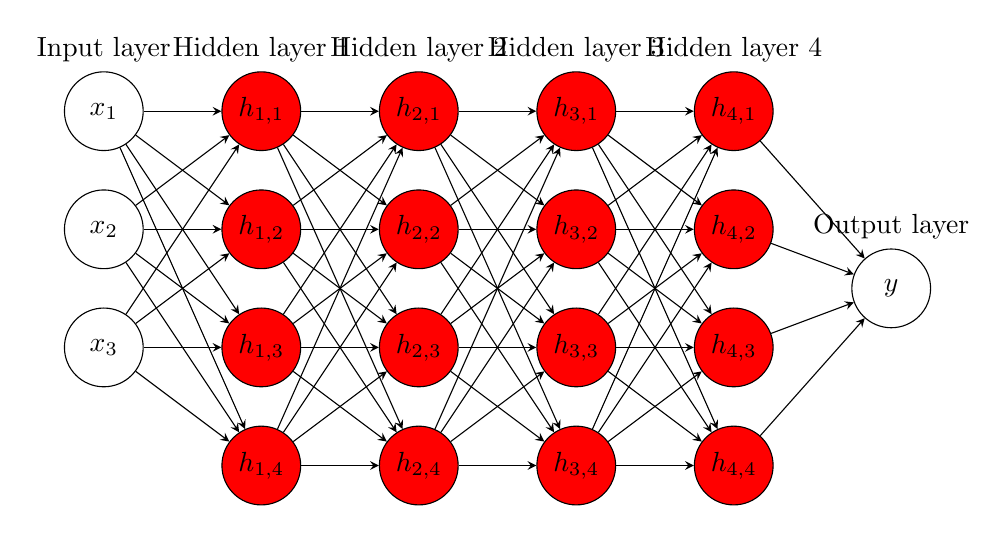
\begin{tikzpicture}[x=1cm, y=1.5cm, >=stealth]
        % Input layer nodes
        \foreach \i in {1,...,3}
        \node[circle, draw=black, fill=white, inner sep=0pt, minimum size=10mm] (I-\i) at (0,-\i) {$x_\i$};

        % Hidden layer nodes
        \foreach \i in {1,...,4}
        \node[circle, draw=black, fill=red, inner sep=0pt, minimum size=10mm] (H1-\i) at (2,-\i) {$h_{1,\i}$};
        \foreach \i in {1,...,4}
        \node[circle, draw=black, fill=red, inner sep=0pt, minimum size=10mm] (H2-\i) at (4,-\i) {$h_{2,\i}$};
        \foreach \i in {1,...,4}
        \node[circle, draw=black, fill=red, inner sep=0pt, minimum size=10mm] (H3-\i) at (6,-\i) {$h_{3,\i}$};
        \foreach \i in {1,...,4}
        \node[circle, draw=black, fill=red, inner sep=0pt, minimum size=10mm] (H4-\i) at (8,-\i) {$h_{4,\i}$};

        % Output layer nodes
        \node[circle, draw=black, fill=white, inner sep=0pt, minimum size=10mm] (O) at (10,-2.5) {$y$};

        % Connections
        \foreach \source in {1,...,3}
        \foreach \dest in {1,...,4}
        \draw[->] (I-\source) -- (H1-\dest);
        \foreach \source in {1,...,4}
        \foreach \dest in {1,...,4}
        \draw[->] (H1-\source) -- (H2-\dest);
        \foreach \source in {1,...,4}
        \foreach \dest in {1,...,4}
        \draw[->] (H2-\source) -- (H3-\dest);
        \foreach \source in {1,...,4}
        \foreach \dest in {1,...,4}
        \draw[->] (H3-\source) -- (H4-\dest);
        \foreach \source in {1,...,4}
        \draw[->] (H4-\source) -- (O);

        % Labels
        \node[above] at (I-1.north) {Input layer};
        \node[above] at (H1-1.north) {Hidden layer 1};
        \node[above] at (H2-1.north) {Hidden layer 2};
        \node[above] at (H3-1.north) {Hidden layer 3};
        \node[above] at (H4-1.north) {Hidden layer 4};
        \node[above] at (O.north) {Output layer};
    \end{tikzpicture}
    \caption{Neural network with 3 input nodes, 4 hidden layers with 3 nodes each, and 1 output layer with 1 node.}
    \label{fig:neural_network}
\end{figure}

Quali sono i primi problemi che vanno gestiti in questo caso? Abbiamo il
problema che i \textbf{dati sono parole e non numeri}. Quindi dobbiamo
trasformare le parole in numeri.

Ogni parola viene \textbf{trasformato} in un numero. Ci troviamo però con delle
recensioni che sono delle \textbf{sequenze di parole}, e quindi abbiamo delle
\textbf{sequenze di numeri}. La soluzione è quelal di usare un \textbf{set di
    parole codificate.} Mi spiego:

Immaginiamo di avere 10.000 parole encodate. Salvo queste 10.000 parole in un
array e associo ad ogni parola un indice di questo array.

\begin{figure}[H]
    \begin{center}
        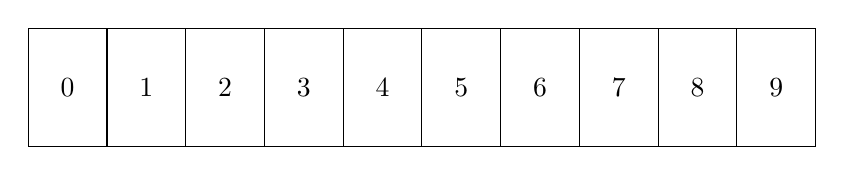
\begin{tikzpicture}[x=1cm, y=1.5cm, >=stealth]
            \draw (0,0) rectangle (10,1);
            \draw (0,0) rectangle (1,1);
            \draw (1,0) rectangle (2,1);
            \draw (2,0) rectangle (3,1);
            \draw (3,0) rectangle (4,1);
            \draw (4,0) rectangle (5,1);
            \draw (5,0) rectangle (6,1);
            \draw (6,0) rectangle (7,1);
            \draw (7,0) rectangle (8,1);
            \draw (8,0) rectangle (9,1);
            \draw (9,0) rectangle (10,1);
            \node at (0.5,0.5) {0};
            \node at (1.5,0.5) {1};
            \node at (2.5,0.5) {2};
            \node at (3.5,0.5) {3};
            \node at (4.5,0.5) {4};
            \node at (5.5,0.5) {5};
            \node at (6.5,0.5) {6};
            \node at (7.5,0.5) {7};
            \node at (8.5,0.5) {8};
            \node at (9.5,0.5) {9};
        \end{tikzpicture}

    \end{center}
\end{figure}

Ora, cosa manca? \textbf{Manca l'ordine}. L'unica cosa che abbiamo è quindi una
indicizzazione delle parole, ma non abbiamo alcuna informazione dell'ordine.
\textbf{Manca anche totalmente la semantica}.

La struttura dell'input è quindi un \textbf{livello con 10.000 nodi di input.s}

\textbf{Input}
\begin{lstlisting}[language=Python]
import numpy as np
def vectorize_sequences(sequences, dimension=10000):
# Create an all-zero matrix of shape (len(sequences), dimension)
results = np.zeros((len(sequences), dimension))
for i, sequence in enumerate(sequences):
    results[i, sequence] = 1. # set specific indices of results[i] to 1s
return results
# Our vectorized training data
x_train = vectorize_sequences(train_data)
# Our vectorized test data
x_test = vectorize_sequences(test_data)

\end{lstlisting}

\textbf{Output}
\begin{lstlisting}[language=Python]
# Our vectorized labels
y_train = np.asarray(train_labels).astype('float32')
y_test = np.asarray(test_labels).astype('float32')

\end{lstlisting}

\subsection{Definizione della Rete Neurale}
\textbf{Codice iniziale della definizione della Rete}

\begin{lstlisting}[language=Python]
    from keras import models
from keras import layers
model = models.Sequential()
model.add(layers.Dense(16, activation='relu', input_shape=(10000,)))
model.add(layers.Dense(16, activation='relu'))
model.add(layers.Dense(1, activation='sigmoid'))
model.compile(optimizer='rmsprop', 
            loss='binary_crossentropy',
             metrics=['accuracy'])
\end{lstlisting}

Il \textbf{modello sequenziale} è quello migliore da dove iniziare. Cosa
significa però modello sequenziale? Il modello sequenziale ha il concetto di
\textbf{layer}. Ha la funzione \textbf{add} che aggiunge un layer sopra gli
altri layer che sono già esistenti.

\textbf{Primo Layer:}

\textit{layers.Dense}: un layer denso significa che ogni nodo di quel layer è collegato con ogni nodo del layer precedente. \textbf{16} è il numero di neuroni che si vogliono attivare in quel layer.
input\_shape è la dimensione dell'input. \textbf{10000} è la dimensione dell'input. Notare che si ha una \textbf{virgola} nell'input dopo il 10.000 e indica che \textit{che stiamo aspettando una sequenza di vettori, ognuno di dimensione 10.000}
Cioè, praticamente stiamo dicendo \textbf{10.000} sono le parole per ogni recensione, e con la virgola stiamo dicendo che \textbf{non sappiamo quante recensioni abbiamo}.E' comodo quando non abbiamo un numero
fisso di example del dataset da processare.

\textbf{Quante connessioni ci sono?} \[16 \cdot 10000 + 16 = 160016\] dove sono 16 i bias.

\textbf{Cosa significa relu?} ReLu è la funzione di attivazione.

\begin{tikzpicture}
    \begin{axis}[
            xlabel={x},
            ylabel={y},
            xmin=-10, xmax=10,
            ymin=-10, ymax=10,
            xtick={-10,-5,0,5,10},
            ytick={-10,-5,0,5,10},
            legend pos=north east,
            ymajorgrids=true,
            grid style=dashed,
            thick
        ]
        \addplot[
            color=custompurple,
            thick
        ]
        coordinates {
                (-10,0)(-9,0)(-8,0)(-7,0)(-6,0)(-5,0)(-4,0)(-3,0)(-2,0)(-1,0)(0,0)(1,1)(2,2)(3,3)(4,4)(5,5)(6,6)(7,7)(8,8)(9,9)(10,10)
            };
    \end{axis}
\end{tikzpicture}

E' una funzione di attivazione artificiale che fino a 0 è 0, e poi cresce
linearmente. E' una funzione che si usa molto in deep learning.

\textbf{Secondo layer}:

Nel secondo layer abbiamo altri \textbf{16} nodi connessi con i precedenti 16
nodi. In tutto abbiamo \[16 \cdot 16 + 16 = 272\] connessioni, con 16 che sono i bias.

\textbf{Layer di output}:

In questo layer abbiamo un unico nodo connesso con i 16 nodi precedenti. In
tutto abbiamo \[16 \cdot 1 + 1 = 17\] connessioni, con 1 che è il bias. La funzione di attivazioe è la
\textbf{sigmoid}, che è una funzione che ha range $[0,1]$ che indica la
probabilità che il dato appartenga alla classe 1.

Diciamo che è stato osservato che la \textit{sigmoid è meglio nell'output}.
Perché? Eh funziona cosi a quanto pare lol.

\begin{tikzpicture}
    \begin{axis}[
            xlabel=$x$,
            ylabel=$\sigma(x)$,
            xmin=-6, xmax=6,
            ymin=-0.1, ymax=1.1,
            samples=100,
            thick,
            every axis plot/.append style={line width=1.5pt}
        ]
        \addplot[custompurple,domain=-6:6] {1/(1+exp(-x))};
    \end{axis}
\end{tikzpicture}

\textbf{Compilazione del modello}

In questa sezione si definisce il \textbf{loss} e l'\textbf{optimizer}.

L'ottimizzatore sarebbe, praticamente, la \textit{discesa del gradiente}. Ci
sono vari ottimizzatori ed è molto buono per te stesso provare gli
ottimizzatori e vedere quale funziona meglio per il tuo problema. Letteralmente
il deep learning :) Per quanto riguarda la loss abbiamo visto nella scorsa
sezione le funzioni di loss che conosciamo.

La \textbf{metrica} è quella che viene usata per valutare effettivamente il
modello. In questo caso si usa l'\textbf{accuracy} che praticamente è la
percentuale di classificazioni corrette.

\subsection{Plotting del modello}

E' un plotting molto base e non molto fancy, ma fa il suo lavoro diciamo
\begin{lstlisting}[language=Python]
from keras.utils import plot_model
plot_model(model, show_shapes=True, show_layer_names=True)
    
\end{lstlisting}

\begin{figure}[H]
    \centering
    \includegraphics[width=0.8\linewidth]{images/plot res.png}
    \caption{Plotting del modello.}
    \label{fig:plot_model}
\end{figure}

\subsection{Training del modello e valutazione}

Entra in gioco il concetto di \textbf{validation set}.

\subsubsection{Validation Set}
Quando ho un modello, come faccio a sapere se la rete che sto allenando si sta
allenando in modo corretto? Tutto questo sapendo che \textbf{non abbiamo
    accesso al test set}. Pensiamo al \textbf{training set} e pensiamo ad un altro
\textbf{split} interno al training set:
\begin{itemize}
    \item Training set parziale
    \item Validation set
\end{itemize}

Quindi se avessimo 50.000 di grandezza del dataset:
\begin{itemize}
    \item 25.000 test set
    \item 25.training set
          \begin{itemize}
              \item 10.000 validation set
              \item 15.000 training set parziale
          \end{itemize}
\end{itemize}

\begin{lstlisting}
x_val = x_train[:10000]
partial_x_train = x_train[10000:]
y_val = y_train[:10000]
partial_y_train = y_train[10000:]

\end{lstlisting}

Praticamente è come se usassimo il validation come se fosse un test set. Quindi
andremo a plottare 2 curve:
\begin{itemize}
    \item La loss sulle epoche
    \item L'accuracy sulle epoche
\end{itemize}

\textbf{La loss} ci da un'idea di quanto il modello si sta allenando bene. Se ci sono problemi, la figura è strana e non segue un andamento corretto, si modifica.
Ma la cosa importante è la \textbf{validation accuracy}, che DEVE essere crescere in modo monotono e deve avvicinarsi a 1 il più possibile.

%grafico loss
\begin{figure}[H]
    \centering
    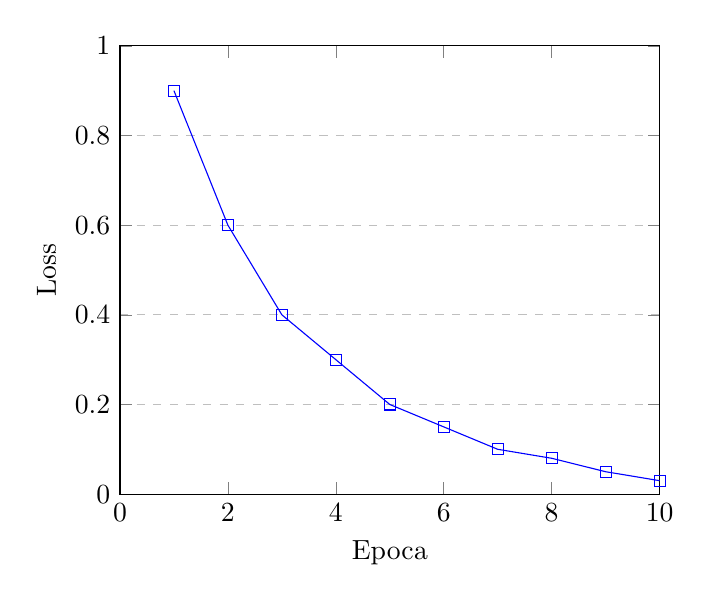
\begin{tikzpicture}
        \begin{axis}[
                xlabel={Epoca},
                ylabel={Loss},
                xmin=0, xmax=10,
                ymin=0, ymax=1,
                xtick={0,2,4,6,8,10},
                ytick={0,0.2,0.4,0.6,0.8,1},
                legend pos=north east,
                ymajorgrids=true,
                grid style=dashed,
            ]
            \addplot[
                color=blue,
                mark=square,
            ]
            coordinates {
                    (1,0.9)(2,0.6)(3,0.4)(4,0.3)(5,0.2)(6,0.15)(7,0.1)(8,0.08)(9,0.05)(10,0.03)
                };
        \end{axis}
    \end{tikzpicture}
    \caption{Grafico di una curva di loss che diminuisce all'aumentare delle epoche.}
    \label{fig:loss_curve}
\end{figure}

%grafico accuracy
\begin{figure}[H]
    \centering
    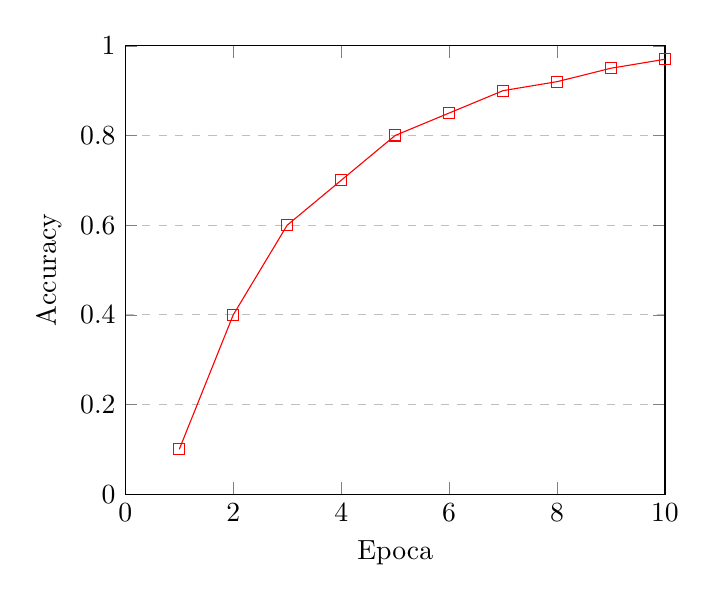
\begin{tikzpicture}
        \begin{axis}[
                xlabel={Epoca},
                ylabel={Accuracy},
                xmin=0, xmax=10,
                ymin=0, ymax=1,
                xtick={0,2,4,6,8,10},
                ytick={0,0.2,0.4,0.6,0.8,1},
                legend pos=north east,
                ymajorgrids=true,
                grid style=dashed,
            ]
            \addplot[
                color=red,
                mark=square,
            ]
            coordinates {
                    (1,0.1)(2,0.4)(3,0.6)(4,0.7)(5,0.8)(6,0.85)(7,0.9)(8,0.92)(9,0.95)(10,0.97)
                };
        \end{axis}
    \end{tikzpicture}
    \caption{Grafico di una curva di accuracy che aumenta all'aumentare delle epoche.}
    \label{fig:accuracy_curve}
\end{figure}

Ma anche se avessimo queste curve inìcon questa conformazione, \textbf{ancora
    non ci dice niente}. Il validation è in un senso insensato per l'output. Ciò
che importerà sarà il \textbf{test set} che non è stato usato per il training.

\textbf{Training code}

\begin{lstlisting}[language=Python]
history = model.fit(partial_x_train,
            partial_y_train,
            epochs=20,
            batch_size=512,
            validation_data=(x_val, y_val))
\end{lstlisting}

\textbf{Plotting delle curve}

Notare che questo è un plotting molto base e non molto fancy, e in futuro
utilizzeremo \textbf{Tensorboard} che aggiornerà in tempo reale i grafici

\begin{lstlisting}[language=Python]
import matplotlib.pyplot as plt
loss = history.history['loss']
val_loss = history.history['val_loss']
epochs = range(1, len(loss) + 1)
# "bo" is for "blue dot"
plt.plot(epochs, loss, 'bo', label='Training loss')
# b is for "solid blue line"
plt.plot(epochs, val_loss, 'b', label='Validation loss')
plt.title('Training and validation loss')
plt.xlabel('Epochs')
plt.ylabel('Loss')
plt.legend()
plt.show()
\end{lstlisting}

Notare che \textit{history} è un dizionario e si può accedere come indicato a
riga \textit{1 e 2} come accedere a loss e val\_loss.
\begin{figure}[H]
    \centering
    \includegraphics[width=0.8\linewidth]{images/wrong network.png}
    \caption{Rete sbagliata}
    \label{fig:loss}
\end{figure}

Un grafico del genere ci mostra una rete che \textbf{funziona male}!.

\begin{lstlisting}[language=Python]
plt.clf() # clear figure
acc = history_dict['binary_accuracy']
val_acc = history_dict['val_binary_accuracy']
plt.plot(epochs, acc, 'bo', label='Training acc')
plt.plot(epochs, val_acc, 'b', label='Validation acc')
plt.title('Training and validation accuracy')
plt.xlabel('Epochs')
plt.ylabel('Accuracy')
plt.legend()
plt.show()

\end{lstlisting}

\begin{figure}[H]
    \centering
    \includegraphics[width=0.8\linewidth]{images/overfitting.png}
    \caption{Overfitting}
    \label{fig:overfitting}
\end{figure}

In questo caso la rete ha un problema di \textbf{overfitting!}.

\subsection{Prediction}
\begin{lstlisting}
model.predict(x_test)
\end{lstlisting}
\[array([[ 0.91966152], [ 0.86563045], [ 0.99936908], ..., [ 0.45731062], [
                    0.0038014 ], [ 0.79525089]], dtype=float32\]

\subsection{Come risolvere problemi di accuracy bassa?}
Se quando andiamo a fare la validazione della nostra rete, come sappiamo come
modificare qualcosa per rendere la rete migliore? Ci sono alcuni approcci per
farlo:
\begin{itemize}
    \item Cambiare la topologia
    \item Diminuire le epoche
    \item Cambiare il numero di nodi per qualche layer
    \item FORSE cambiare anche il learning rate
\end{itemize}

Si noti che facendo questo vanno interpretati i grafici per capire come sta
andando la rete. Quando cominciamo a vedere che la \textbf{validation accuracy}
\textbf{NON STA SOLAMENTE CRESCENDO} ma ci sono dei punti in cui diminuisce,
siamo sicuri che \textbf{c'è qualche problema di mezzo.} Bisogna capire anche
su cosa lavorare. Se cambiando i dati spesso la \textbf{validation accuracy}
mostra problemi, allora bisogna lavorare per quello e cercare di trovare un
modo per fare in modo che il problema non si presenti.

\textbf{RECAPPONE}: Se notiamo che nella LOSS ci sono problemi, possiamo tunare il \textbf{learning rate} e altri
parametri per cercare di risolvere questi problemi. Ma la cosa più importante è \textbf{la metrica}. Se notiamo che
la \textbf{metrica non rispecchia un andamento di effettivo apprendimento}, capiamo che la rete non si sta comportando nel modo corretto
e non sta funzionando.

\subsection{Early Stopping}

E' un metodo che consiste nel vedere quando \textbf{la loss} comincia ad avere
dei comportamenti sospetti. Quando si \textbf{ferma} la rete in un dato
momento, si impedisce alla rete di \textbf{overfittare} nella maggior parte dei
casi.

\section{Classificazione Multiclasse}

Questa sezione sarà molto corta, poiché praticamente è la stessa cosa della
classificazione binaria, ma il layer finale della rete non sarà composto da un
solo nodo, ma da \textbf{un numero di nodi pari al numero di classi da
    classificare}.

\subsection{Descrizione del dataset - Reuters}

Il dataset che verrà utilizzato è il \textbf{Reuters Dataset}, che è un dataset
di \textbf{news} che sono state classificate in \textbf{46 categorie}. Ogni
categoria ha almeno 10 esempi nel training set.

\textbf{Preprocessing dell'input}

\begin{lstlisting}[language=Python]
import numpy as np
def vectorize_sequences(sequences, dimension=10000):
    results = np.zeros((len(sequences), dimension))
    for i, sequence in enumerate(sequences):
        results[i, sequence] = 1.
    return results
# Our vectorized training data
x_train = vectorize_sequences(train_data)
# Our vectorized test data
x_test = vectorize_sequences(test_data)
\end{lstlisting}

\subsubsection{Come processiamo l'output?}

Nel deep learning, \textbf{gli output categorici} non vengono mai mappati ad
una scala numerica. Si utilizza una tecnica che si chiama \textbf{one hot
    encoding}.

\textbf{One Hot Encoding}:

Consiste nel creare tante variabili numeriche quanti sono i valori della
variabile categorica, e per quel dato example viene assegnato
\begin{itemize}
    \item 1: se il valore della variabile categorica è quello
    \item 0: se il valore della variabile categorica non è quello, quindi in tutti gli altri casi
\end{itemize}

Da notare che il one hot encoding viene fatto sia per le labels di output, ma
non è sbagliato farlo anche per gli attributi in alcuni casi.

\begin{lstlisting}[language=Python]
def to_one_hot(labels, dimension=46):
    results = np.zeros((len(labels), dimension))
    for i, label in enumerate(labels):
        results[i, label] = 1.
    return results
# Our vectorized training labels
one_hot_train_labels = to_one_hot(train_labels)
# Our vectorized test labels
one_hot_test_labels = to_one_hot(test_labels)

#OPPURE ALLO STESSO MODO

from keras.utils.np_utils import to_categorical

one_hot_train_labels = to_categorical(train_labels)
one_hot_test_labels = to_categorical(test_labels)
\end{lstlisting}

\textbf{Nota}: nel one hot encoding DOBBIAMO AVERE 1 SOLO VALORE per il dato example, e tutti gli altri non devono essere attivi.
La domanda è, quindi, \textbf{quale activation function usiamo?}

\textit{Immaginiamo questa situazione}: Abbiamo $y_1, y_2, y_3$ che sono i valori di output. Vogliamo solamente uno dei tre.
Se normalizzassimo i dati in questo modo:
\begin{itemize}
    \item $p_1 = \frac{y_1}{y_1+y_2+y_3}$
    \item $p_2 = \frac{y_2}{y_1+y_2+y_3}$
    \item $p_3 = \frac{y_3}{y_1+y_2+y_3}$
\end{itemize}

E se sommiamo $p_1+p_2+p_3$ otteniamo 1. Quindi, in questo caso, possiamo usare
la \textbf{softmax} come activation function.

\subsubsection{Softmax activation function}

Se prendiamo un vettore $\vec{y} = (y_1, y_2, y_3)$, la softmax è definita
come:

\begin{equation}
    S(y_i) = \frac{e^{y_i}}{\sum_{j=1}^{3} e^{y_j}}
\end{equation}

In output abbiamo: $\vec{p} = (p_1, p_2, p_3)$, dove $p_i$ è la probabilità che
il dato example appartenga alla classe $i$.

Nota: quando dividiamo qualcosa, abbiamo \textbf{sempre} un problema riguardo
la stabilità numerica. La divisione è molto critica, poiché \textbf{potrebbe
    essere vicina a 0}. Sappiamo che se usiamo $e^y_1 + e^y_2 + e^y_3$
difficilmente si avvicina a 0.

\begin{lstlisting}[language=Python]
    from keras import models
    from keras import layers
    model = models.Sequential()
    model.add(layers.Dense(64, activation='relu', input_shape=(10000,)))
    model.add(layers.Dense(64, activation='relu'))
    model.add(layers.Dense(46, activation='softmax'))
    model.compile(optimizer='rmsprop',
                loss='categorical_crossentropy',
                metrics=['accuracy'])
\end{lstlisting}

\textbf{Nota:} Dobbiamo avere un numero di nodi di output quanto il numero di classi,
ma \textbf{altra cosa}, il numero di nodi interni deve essere sicuramente
maggiore di 46, altrimenti ci sarebbe una perdita di informazioni.

\textbf{Nota 2:} La funzione di attivazione dell'ultimo layer è una \textbf{softmax}.

\textbf{Validation set e Training set}
\begin{lstlisting}[language=Python]
   
x_val = x_train[:1000]
partial_x_train = x_train[1000:]
y_val = one_hot_train_labels[:1000]
partial_y_train = one_hot_train_labels[1000:]
history = model.fit(partial_x_train,
                partial_y_train,
                epochs=20,
                batch_size=512,
                validation_data=(x_val, y_val))
\end{lstlisting}

\textbf{Loss}

\begin{lstlisting}[language=Python]
import matplotlib.pyplot as plt
loss = history.history['loss']
val_loss = history.history['val_loss']
epochs = range(1, len(loss) + 1)
plt.plot(epochs, loss, 'bo', label='Training loss')
plt.plot(epochs, val_loss, 'b', label='Validation loss')
plt.title('Training and validation loss')
plt.xlabel('Epochs')
plt.ylabel('Loss')
plt.legend()
plt.show()
\end{lstlisting}

\textbf{Accuracy}

\begin{lstlisting}[language=Python]
plt.clf() # clear figure
acc = history.history['acc']
val_acc = history.history['val_acc']
plt.plot(epochs, acc, 'bo', label='Training acc')
plt.plot(epochs, val_acc, 'b', label='Validation acc')
plt.title('Training and validation accuracy')
plt.xlabel('Epochs')
plt.ylabel('Acc')
plt.legend()
plt.show()

\end{lstlisting}

\textbf{Nota:} L'accuracy è importante dipendentemente dall'utilizzo che bisogna farne.
Ad esempio, \textit{in ambito medico} vogliamo \textbf{minimizzare i falsi negativi}. Questo implica
che la misura che usiamo dipende dall'applicazione che se ne fa.